% --- APPENDIX: FOURIER KDE ---
\appendix % Đánh dấu bắt đầu phụ lục (Reset số trang hoặc đổi màu)

% --- SLIDE A1: THE THEORETICAL FOUNDATION ---
\begin{frame}{Appendix A: Beyond Gaussian (Fourier Approach)}
    \small
    \textbf{Motivation:} Standard KDE struggles with bandwidth matrices ($\mathbf{H}$) in high dimensions. Is there a better way?

    \vspace{0.5em}
    \begin{block}{The Fourier Integral Theorem (Identity)}
        Any square-integrable function $f(\vect{x})$ can be reconstructed \textbf{exactly} via:
        \begin{equation}
            f(\vect{x}) = \lim_{R \to \infty} \frac{1}{\pi^d} \int_{\mathbb{R}^d} \prod_{j=1}^{d} \frac{\sin(R(x_j - t_j))}{x_j - t_j} f(\vect{t}) d\vect{t}
        \end{equation}
    \end{block}

    \vspace{0.5em}
    \begin{columns}[c]
        \begin{column}{0.6\textwidth}
            \textbf{The Estimator (Monte Carlo approx):}
            $$ \hat{f}_{n,R}(\vect{x}) = \frac{1}{n \pi^d} \sum_{i=1}^{n} \prod_{j=1}^{d} \underbrace{\frac{\sin(R(x_j - X_{ij}))}{x_j - X_{ij}}}_{\text{Sinc Kernel}} $$
        \end{column}
        \begin{column}{0.4\textwidth}
            \begin{alertblock}{Key Difference}
                \centering \footnotesize
                It uses the \textbf{Sinc Kernel} instead of Gaussian.
                \\ $\text{sinc}(u) = \frac{\sin(u)}{u}$
            \end{alertblock}
        \end{column}
    \end{columns}
\end{frame}

% --- SLIDE A2: THE "KILLER FEATURE" (AUTOMATIC DEPENDENCE) ---
\begin{frame}{Appendix B: The "Magic" of Fourier KDE}
    \textbf{The Big Question:} How does it handle correlation without a matrix $\mathbf{H}$?

    \vspace{1em}
    \begin{columns}[T]
        % --- LEFT: GAUSSIAN STRUGGLE ---
        \begin{column}{0.48\textwidth}
            \begin{block}{1. Gaussian KDE (Traditional)}
                \small
                To capture correlation, we \textbf{MUST} estimate a full matrix $\mathbf{H}$ (or $\mathbf{\Sigma}^{-1}$).
                \vspace{0.5em}
                \begin{itemize}
                    \item $\prod K(x_j)$ (Diagonal) $\to$ \textcolor{red}{Fails (Axis-aligned)}.
                    \item Full $\mathbf{H}$ $\to$ \textcolor{orange}{Expensive ($O(d^2)$)}.
                \end{itemize}
            \end{block}
        \end{column}

        % --- RIGHT: FOURIER MAGIC ---
        \begin{column}{0.48\textwidth}
            \onslide<2->{
                \begin{alertblock}{2. Fourier KDE (Advanced)}
                    \small
                    \textbf{Theorem:} A simple product of 1D Sinc kernels \textbf{automatically} recovers the joint density structure.
                    \vspace{0.5em}
                    \begin{itemize}
                        \item \textbf{No Matrix needed!} Just a scalar $R$.
                        \item Captures rotation/correlation natively via the Fourier domain.
                    \end{itemize}
                \end{alertblock}
            }
        \end{column}
    \end{columns}

    \vspace{1em}
    \centering
    \onslide<3->{
        \textbf{\textcolor{darkred}{Verdict:}} Fourier KDE bypasses the "Bandwidth Matrix Selection" headache entirely.
    }
\end{frame}

% --- SLIDE A3: PERFORMANCE & CONVERGENCE ---
\begin{frame}{Appendix C: Performance Superiority}
    \small
    Why should we care? Because it converges faster.

    \vspace{1em}
    \begin{columns}[c]
        \begin{column}{0.5\textwidth}
            \textbf{Convergence Rate (MISE):}
            \vspace{0.5em}
            \begin{itemize}
                \setlength\itemsep{1em}
                \item \textbf{Standard KDE:}
                $$ O(n^{-4/(4+d)}) $$
                \textit{(Suffer from Curse of Dimensionality)}

                \item \textbf{Fourier KDE (Supersmooth):}
                $$ \alert{O(n^{-1} (\log n)^k)} $$
                \textit{(Almost parametric rate $1/n$!)}
            \end{itemize}
        \end{column}

        \begin{column}{0.5\textwidth}
            \centering
            % Vẽ minh họa tốc độ hội tụ đơn giản
            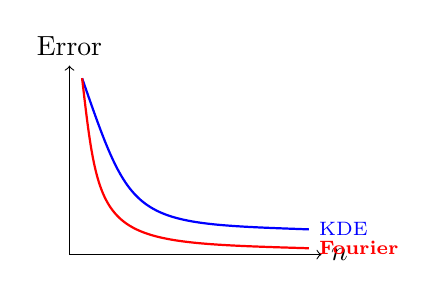
\begin{tikzpicture}[scale=0.8]
                \draw[->] (0,0) -- (4,0) node[right] {$n$};
                \draw[->] (0,0) -- (0,3) node[above] {Error};
                \draw[thick, blue] (0.2, 2.8) .. controls (1, 0.5) .. (3.8, 0.4) node[right] {\scriptsize KDE};
                \draw[thick, red] (0.2, 2.8) .. controls (0.5, 0.2) .. (3.8, 0.1) node[right] {\scriptsize \textbf{Fourier}};
            \end{tikzpicture}
            \vspace{0.5em}
            \captionof{figure}{\scriptsize Faster error decay}
        \end{column}
    \end{columns}

    \vspace{1em}
    \footnotesize
    \textit{Source: Ho, N., \& Walker, S. G. (2021). Multivariate Smoothing via the Fourier Integral Theorem.}
\end{frame}